\documentclass[../main.tex]{subfiles}

\begin{document}
In questa sezione si analizzano alcune delle librerie scelte per la sperimentazione del paradigma FRP in Scala. Aspetti cruciali dell'analisi delle librerie sono la correttezza rispetto la definizione del paradigma FRP (discussa nel capitolo 2), lo stato attuale della libreria (active, maintenance o EOL) ed il supporto a Scala. La sperimentazione è stata effettuata sviluppando gli stessi esempi con le diverse librerie in analisi: \textit{Sodium}, \textit{Reactify}. Gli esempi sviluppati sono i seguenti:
\begin{itemize}
    \item Sensore di temperatura (\textit{XThermalManagerExample}): flusso di rilevamenti simulati di sensori di temperatura e lavorazioni sui valori per estrarre altri valori come temperatura media e spikes.
    \begin{figure}[H]
        \centering
        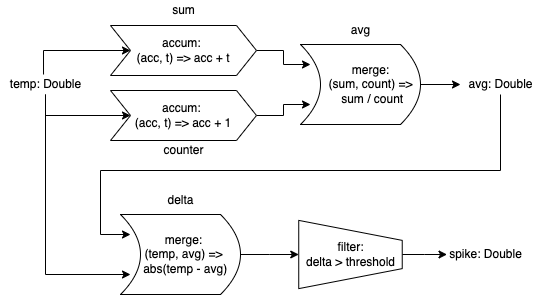
\includegraphics[width=0.9\textwidth]{img/frp-scala-Page-3.drawio.png}
        \caption{Parte del grafo delle dipendenze: temperatura media e spikes}
    \end{figure}
    \item Contatore/ticker (\textit{XTimeFlowExample}): flusso di cambiamenti al valore del contatore, al quale è associata come reazione il calcolo dei millisecondi trascorsi e la stampa del valore.
    \begin{figure}[H]
        \centering
        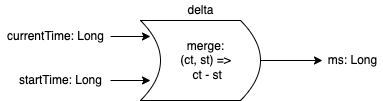
\includegraphics[width=0.7\textwidth]{img/frp-scala-Page-4.drawio.png}
        \caption{Grafo delle dipendenze: timer}
    \end{figure}
\end{itemize}

\section{Sodium}
La libreria open-source Sodium è stata progettata e sviluppata da Stephen Blackheath e Anthony Jones (più altri collaboratori) per fornire una libreria production-ready in diversi linguaggi, tra cui Scala, per promuovere la vera definizione del paradigma FRP e per realizzare un riferimento/benchmark per future librerie.

\begin{table}[H]
\centering
\begin{tabular}{|c|c|}
     \hline
     Repository & https://github.com/SodiumFRP/sodium \\
     \hline
     Versione Latest Release & 1.2.0 \\
     \hline
     Data Latest Release & Ottobre 2019 \\
     \hline
     Data Latest Commit & 3 Febbraio 2020 \\
     \hline
     Supporto Scala & 2.12 \\
     \hline
     Dipendenza Gradle & nz.sodium:sodium:1.2.0 \\
     \hline
\end{tabular}
\caption{Main Info Libreria Sodium}
\end{table}

Nonostante la libreria sia distribuita tramite il repository Maven Central (\url{https://mvnrepository.com/artifact/nz.sodium/sodium/1.2.0}) è stato necessario un fork, disponibile al repo \url{https://github.com/paganellif/sodium} per i seguenti motivi:
\begin{enumerate}
    \item Il package jar della libreria disponibile su maven central è ottenuto dalla pacchettizzazione del sorgente Java. Seppur ci sia grande interoperabilità tra Scala e Java non è possibile sfruttare direttamente le features del linguaggio funzionale. 
    \item Creato il jar partendo dal sorgente Scala sono stati risolti errori/warning permettendo alla libreria di supportare anche Scala 2.13.7, versione utilizzata nel progetto.
\end{enumerate}

\subsection{SodiumThermalManagerExample}
L'entità \textit{SodiumTempSensor} modella un sensore di temperatura che, dato in input un range di valori decimali e la frequenza di spike, ovvero la probabilità che una rilevazione della temperatura da parte del sensore sia sbagliata, emette uno stream di valori decimali rappresentanti la temperatura misurata.

\begin{figure}[H]
    \centering
    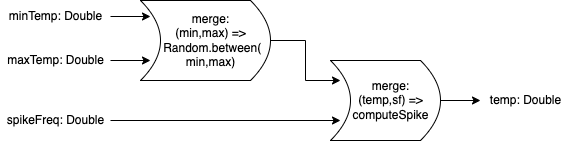
\includegraphics[width=0.9\textwidth]{img/frp-scala-Page-7.drawio.png}
    \caption{Grafo delle dipendenze: TempSensor}
\end{figure}

Lo stream di output del sensore di temperatura, modellato con il costrutto della libreria \textit{Stream[Double]}, rappresenta quindi l'input del componente \textit{SodiumThermalManager}. 

\begin{lstlisting}[language=Javascript, caption=Sodium - Traduzione della parte di grafo delle dipendenze riguardante la temperatura media e gli spike in codice]
implicit class StreamCounter[A](stream: Stream[A]) {
  def count(): Stream[Int] = stream
    .accum(0, (t: A, acc: Int) => acc + 1).updates()
}
  
def sumTemp: Stream[Double] = tempSensor.temp
  .accum(0.0, (t: Double,acc: Double) => acc + t).updates()
    
def firingCount: Stream[Int] = tempSensor.temp.count()

def avgTemp: Stream[Double] = sumTemp.merge(firingCount.map(i => i.toDouble), (s,f) => s / f)

def spikeTemp: Stream[Double] = tempSensor.temp
  .merge(avgTemp, (t, avg) => Math.abs(t - avg)).filter(t => t > thresholdTemp.sample())
\end{lstlisting}

La traduzione in codice del grafo delle dipendenze progettato è possibile grazie alle primitive fornite dalla libreria Sodium, la quale ne aggiunge altre a quelle basiche viste nel capitolo precedente. Un esempio di primitiva aggiuntiva e utilizzata per computare la somma delle temperatura è la primitiva \textit{accum}.

Dato l'output del \textit{SodiumThermalManager} viene registrato come handler una semplice stampa a console di test del valore:
\begin{lstlisting}[language=Javascript, caption=Sodium - Registrazione listeners]
avgTemp.listen(avg => println(s" avg: $avg"))
spikeTemp.listen(spike => println(s"spike: $spike"))
\end{lstlisting}

\subsection{SodiumTimeFlowExample}
Un esempio di test più banale rispetto a quello precedente è la realizzazione di un contatore/ticker: dato il tempo iniziale in millisecondi modifica il valore di una variabile con una certa cadenza periodica, emettendo quindi un flusso di cambiamenti.

\begin{lstlisting}[language=Javascript, caption=Sodium - Esempio completo]
val startTime: Cell[Long] = new Cell(System.currentTimeMillis())
val currentTime: StreamSink[Long] = new StreamSink[Long]()

currentTime.map(ct => ct - startTime.sample())
  .listen(ms => println(s"ms: $ms"))

new Thread(() => {
  while(true) {
    currentTime.send(System.currentTimeMillis())
    sleep(500)
  }
}).start()
\end{lstlisting}

\section{Reactify}
Reactify è una libreria open-source che permette di sviluppare sistemi col paradigma FRP fornendo un insieme limitato di concetti rispetto ad altre librerie come Sodium. Il programma viene espresso in termini di variabili che cambiano (\textit{Var}) o non cambiano (\textit{Val}) valore nel tempo e nel definire una reazione al cambiamento: tutte le primitive tipiche del paradigma FRP non sono fornite dalla libreria, la quale permette di usare qualsiasi funzionalità di Scala direttamente.

\begin{table}[H]
\centering
\begin{tabular}{|c|c|}
     \hline
     Repository & https://github.com/outr/reactify \\
     \hline
     Versione Latest Release & 4.0.6 \\
     \hline
     Data Latest Release & Maggio 2021 \\
     \hline
     Data Latest Commit & 17 Maggio 2021 \\
     \hline
     Supporto Scala & 2.11, 2.12, 2.13, 3 \\
     \hline
     Dipendenza Gradle & com.outr:reactify\_2.13:4.0.6 \\
     \hline
\end{tabular}
\caption{Main Info Libreria Reactify}
\end{table}

\subsection{ReactifyThermalManagerExample}
La struttura e il grado delle dipendenze dell'esempio sviluppato utilizzando la libreria Sodium sono gli stessi per l'esempio sviluppato utilizzando la libreria Reactify. 

A differenza di Sodium, la quale fornisce un ampio set di primitive per la definizione del grafo delle dipendenze, in Reactify esistono solo due concetti principali e due primitive:
\begin{description}
\item[Var] - Equivalente di Cell in Sodium, definisce una variabile che cambia valore nel tempo.
\item[Val] - Equivalente (circa) di Stream in Sodium, definisce la dipendenza tra una o più \textit{Var}. Questo significa che ogni modifica al valore delle dipendenze comporta un ricalcolo e quindi una modifica del valore della \textit{Val}.
\item[Map] - Equivalente della primitiva map in Sodium. Effettua una operazione sul contenuto di una \textit{Var} restituendolo all'interno di una nuova \textit{Var}.
\item[Attach] - Equivalente della primitiva listen in Sodium. Permette di registrare listeners sia a \textit{Var} che \textit{Val}.
\item[Set] - Equivalente della primitiva send in Sodium. Permette di cambiare il valore di una \textit{Var}.
\end{description}

Per poter definire dipendenze più complesse/avanzate rispetto a map/attach è possibile usare qualsiasi costrutto fornito dal linguaggio di programmazione, in questo caso Scala:
\begin{lstlisting}[language=Javascript, caption=Reactify - Traduzione della parte di grafo delle dipendenze riguardante la temperatura media e gli spike in codice e registrazione listeners]
private var _sum: Double = 0.0
val sumTemp: Val[Double] = Val[Double]({ _sum += tempSensor.temp; _sum })

private var _firingCount: Int = 0
val firingCount: Val[Int] = tempSensor.temp.map(t => { _firingCount += 1; _firingCount })

val avgTemp: Val[Double] = Val[Double](sumTemp / firingCount)

val spikeTemp: Val[Option[Double]] = Val[Option[Double]] {
  val delta = Math.abs(tempSensor.temp - avgTemp)
  if(delta > thresholdTemp) Option(delta) else Option.empty
}
. . . .
avgTemp.attach(avg => println(s" avg: $avg"))
spikeTemp.attach(spike => println(s"spike: $spike"))
\end{lstlisting}

\subsection{ReactifyTimeFlowExample}
Come nell'esempio precedente \textit{ReactifyThermalManagerExample} anche in questo caso la struttura e il grafo delle dipendenze adottati sono identici. Anche il numero di righe di codice sviluppate per fare la conversione grafo-codice è lo stesso:
\begin{lstlisting}[language=Javascript, caption=Reactify - Esempio completo]
val startTime: Val[Long] = Val(System.currentTimeMillis())
val currentTime: Var[Long] = Var(System.currentTimeMillis())

val delta: Val[Long] = Val[Long](currentTime - startTime)
delta.attach(ms => println(s"ms: $ms"))

new Thread(() => {
  while(true) {
    currentTime.set(System.currentTimeMillis())
    sleep(500)
  }
}).start()
\end{lstlisting}
La variabile \textit{delta}, definita come \textit{Val}, rappresenta la dipendenza tra il tempo corrente e il tempo iniziale. Il tempo iniziale (\textit{startTime}) è definito come \textit{Val} perchè il suo valore non deve cambiare: non essendoci infatti nessuna dipendenza nella sua definizione è garantito che quel valore è costante nel tempo. Il valore del tempo corrente invece è definito come \textit{Var} perchè viene modificato dal thread utilizzando la primitiva \textit{set}.
\end{document}

